\documentclass[a4paper, 12pt]{article}

\def\languages{french, english}

%%%%%%%%%%%%%%%%%%% Libraries

\input{include/libraries/default.tex}
\input{include/libraries/figures.tex}
\input{include/libraries/informatics.tex}
\input{include/libraries/mathematics.tex}
\input{include/libraries/theorems.tex}
\input{include/libraries/units.tex}

\input{include/languages/french.tex}

%%%%%%%%%%%%%%%%%%% Titlepage

\def\logopath{resources/pdf/logo-uliege.pdf}
\def\toptitle{University of Liège}
\title{Homework 1}
\def\subtitle{Applied digital signal processing}
%\def\authorhead{Author}
\author{
    Quentin \textsc{Graillet} (20164386)\\
    Maxime \textsc{Meurisse} (20161278)\\
    Adrien \textsc{Schoffeniels} (20162843)\\
}
%\def\rightauthorhead{}
%\def\rightauthor{}
\def\context{3\ieme{} year of Bachelor Civil Engineer}
\date{Academic year 2018-2019}

%%%%%%%%%%%%%%%%%%% Others

\NFstyle{matlab}

%%%%%%%%%%%%%%%%%%% Document

\begin{document}
	\input{include/titlepages/default.tex}
	\section{Magnitude response of a filter}
	We consider a filter with the transfer function
	\begin{equation*}
	    H(z) = \dfrac{b_0}{\sbk{1-2r\cos\rbk{\omega_0}z^{-1}+r^2z^{-2}}^K}
	\end{equation*}
	To simplify the study of this function, we consider that it is a cascade of K second-order filters. The function can therefore be decomposed into a product of elementary transfer functions.
	\begin{equation*}
	    H(z) = K\rbk{\dfrac{b_0^{\frac{1}{K}}}{1-2r\cos\rbk{\omega_0}z^{-1}+r^2z^{-2}}}
	\end{equation*}
	We replace the parameters $K$, $r$ and $b_0$ by their value, and we store the coefficients of the numerator in a vector $b$, and those of the denominator in a vector $a$. We define a linearly spaced vector ranging from $-\pi$ to $\pi$ and having \num{500} points. We then use the function \texttt{freqz} of Matlab\footnote{All Matlab codes used are attached to this report.} with these data and we display the result.\par
	The magnitude response for $\omega_0 = \frac{\pi}{3}$ is shown in figure \ref{fig:magnitude_response_a}. To obtain the values of the magnitude in \deci\bel, we multiply all the values $x$ by $10\log_{10}(x)$. The normalized angular frequency is scaled by $\pi$.\par
	\begin{figure}[!ht]
	    \centering
	    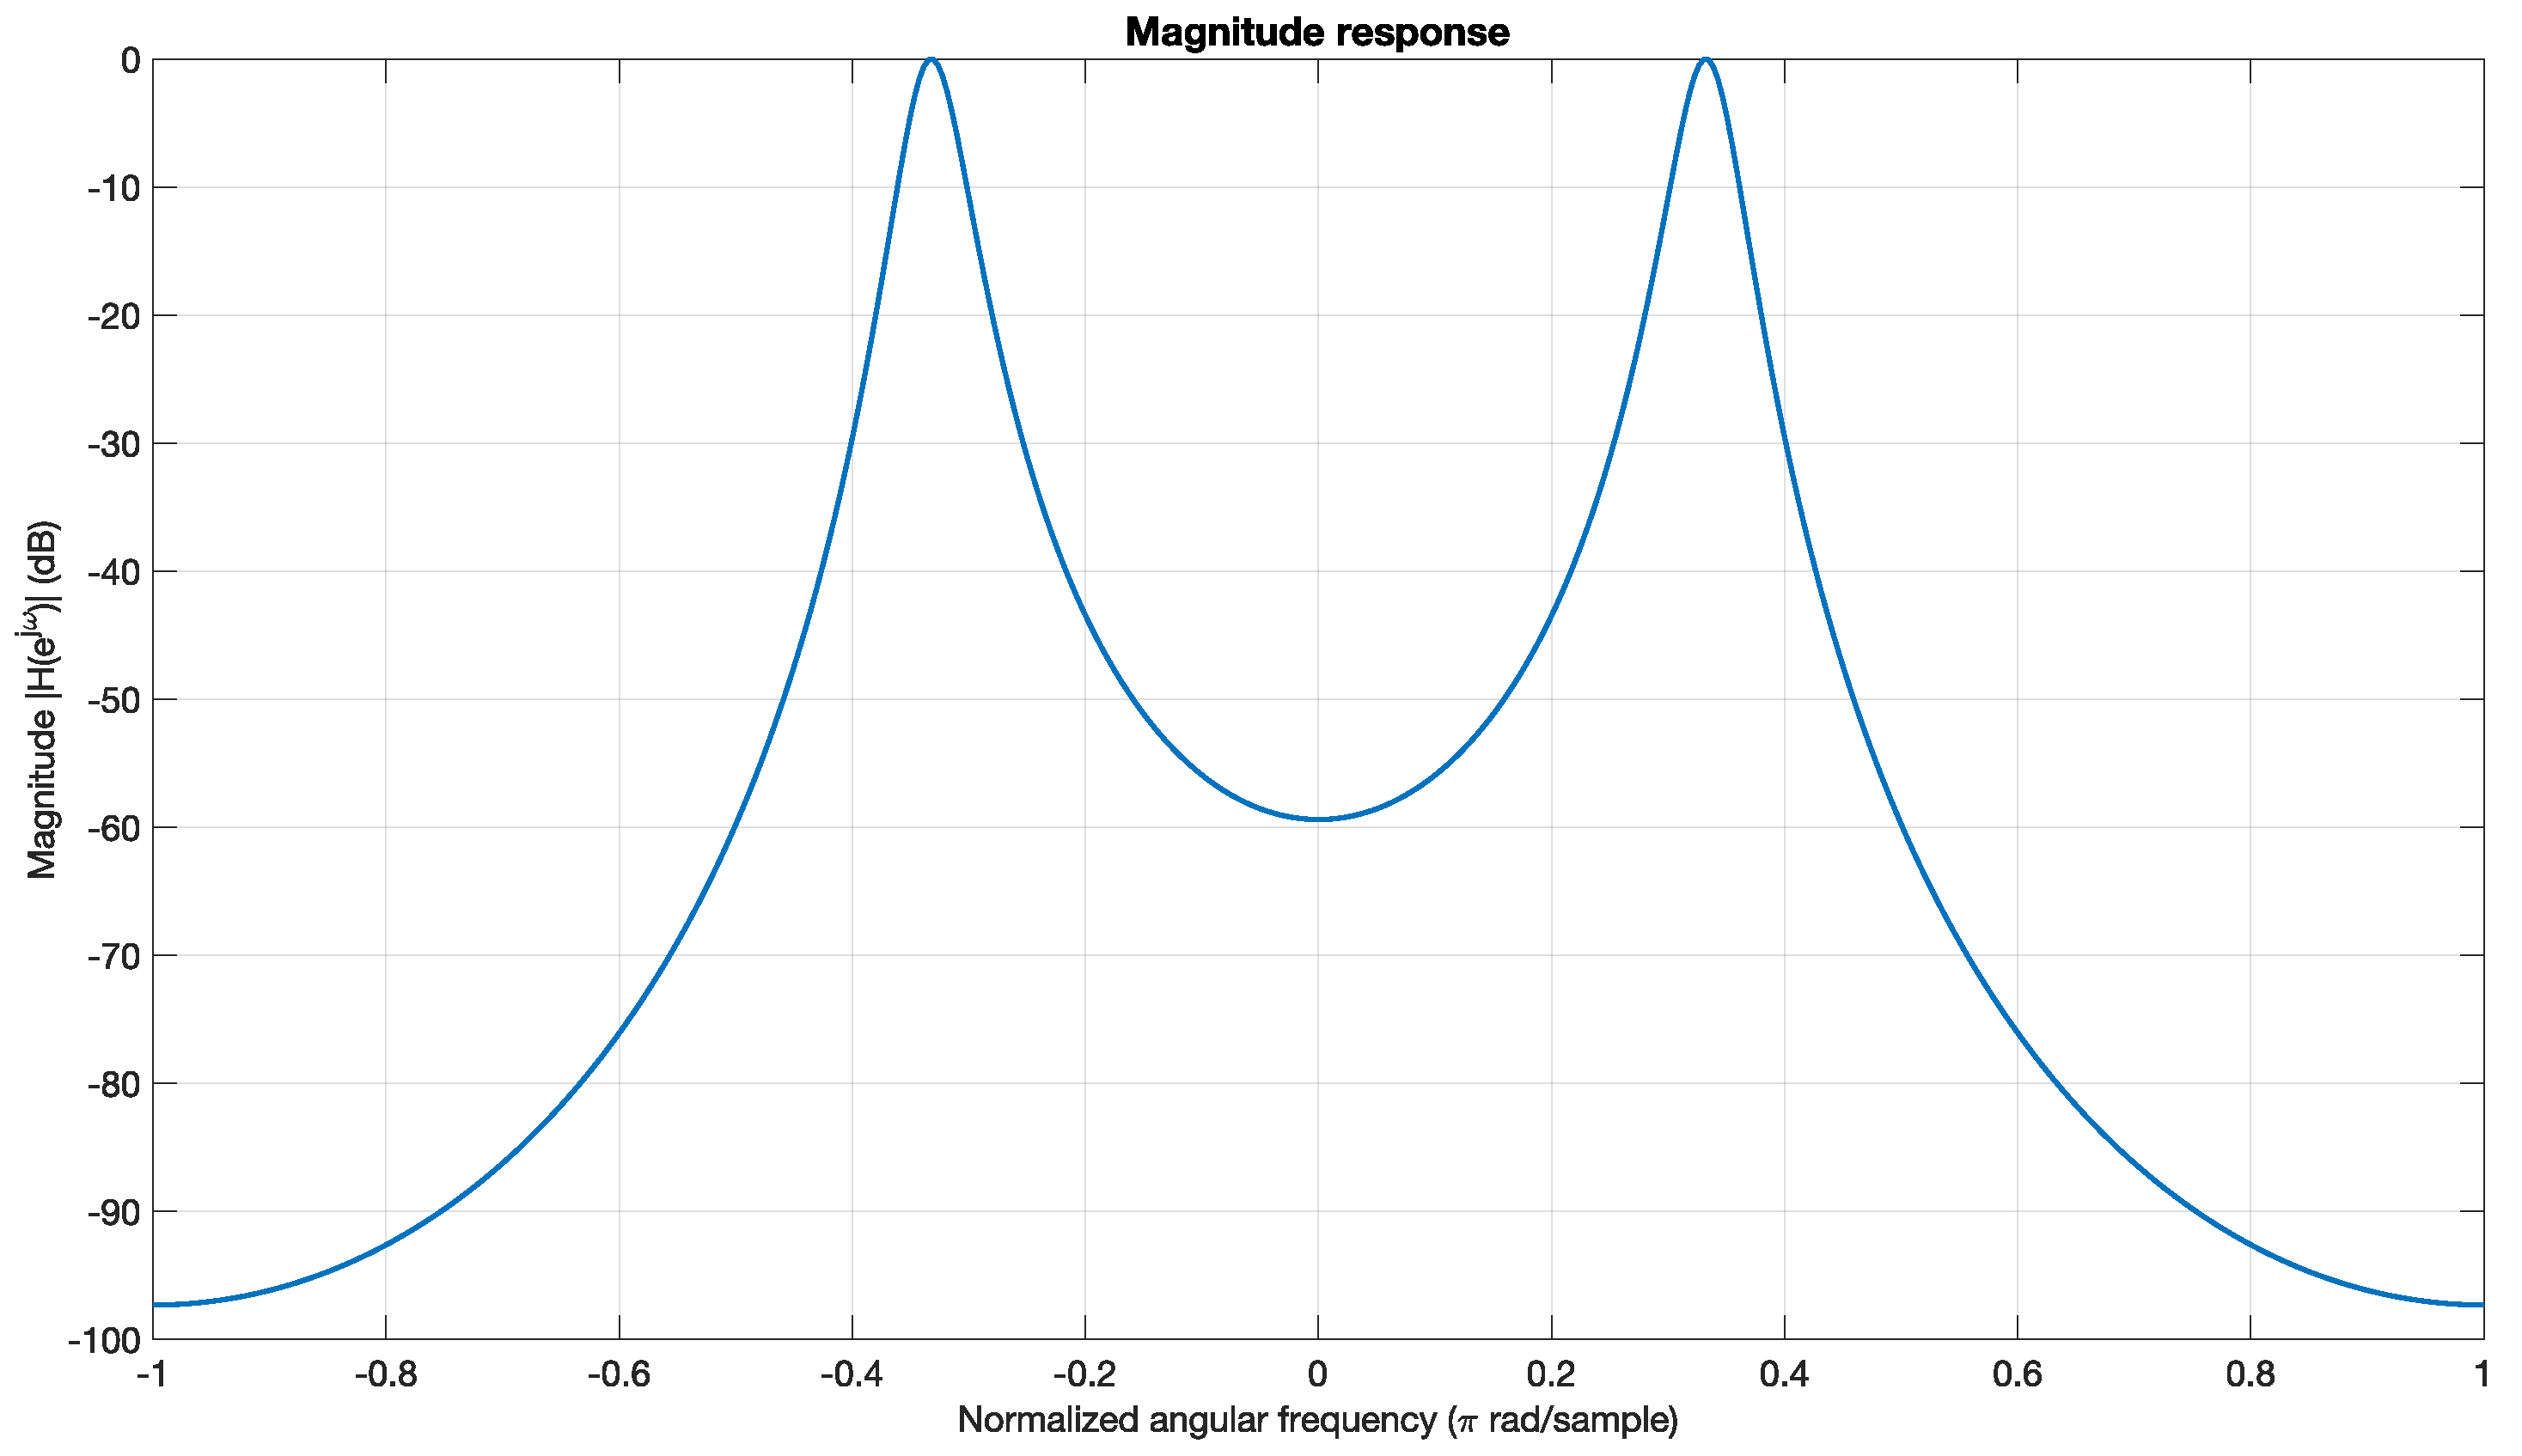
\includegraphics[width=1\textwidth]{resources/pdf/magnitude_response_a.pdf}
	    \caption{Magnitude response $\abs{H(e^{j\omega})}$ for $\omega_0 = \frac{\pi}{3}$.}
	    \label{fig:magnitude_response_a}
	\end{figure}
	We repeat the same procedure for $\omega = \frac{2\pi}{3}$ (figure \ref{fig:magnitude_response_b}).\par
	\begin{figure}[!ht]
	    \centering
	    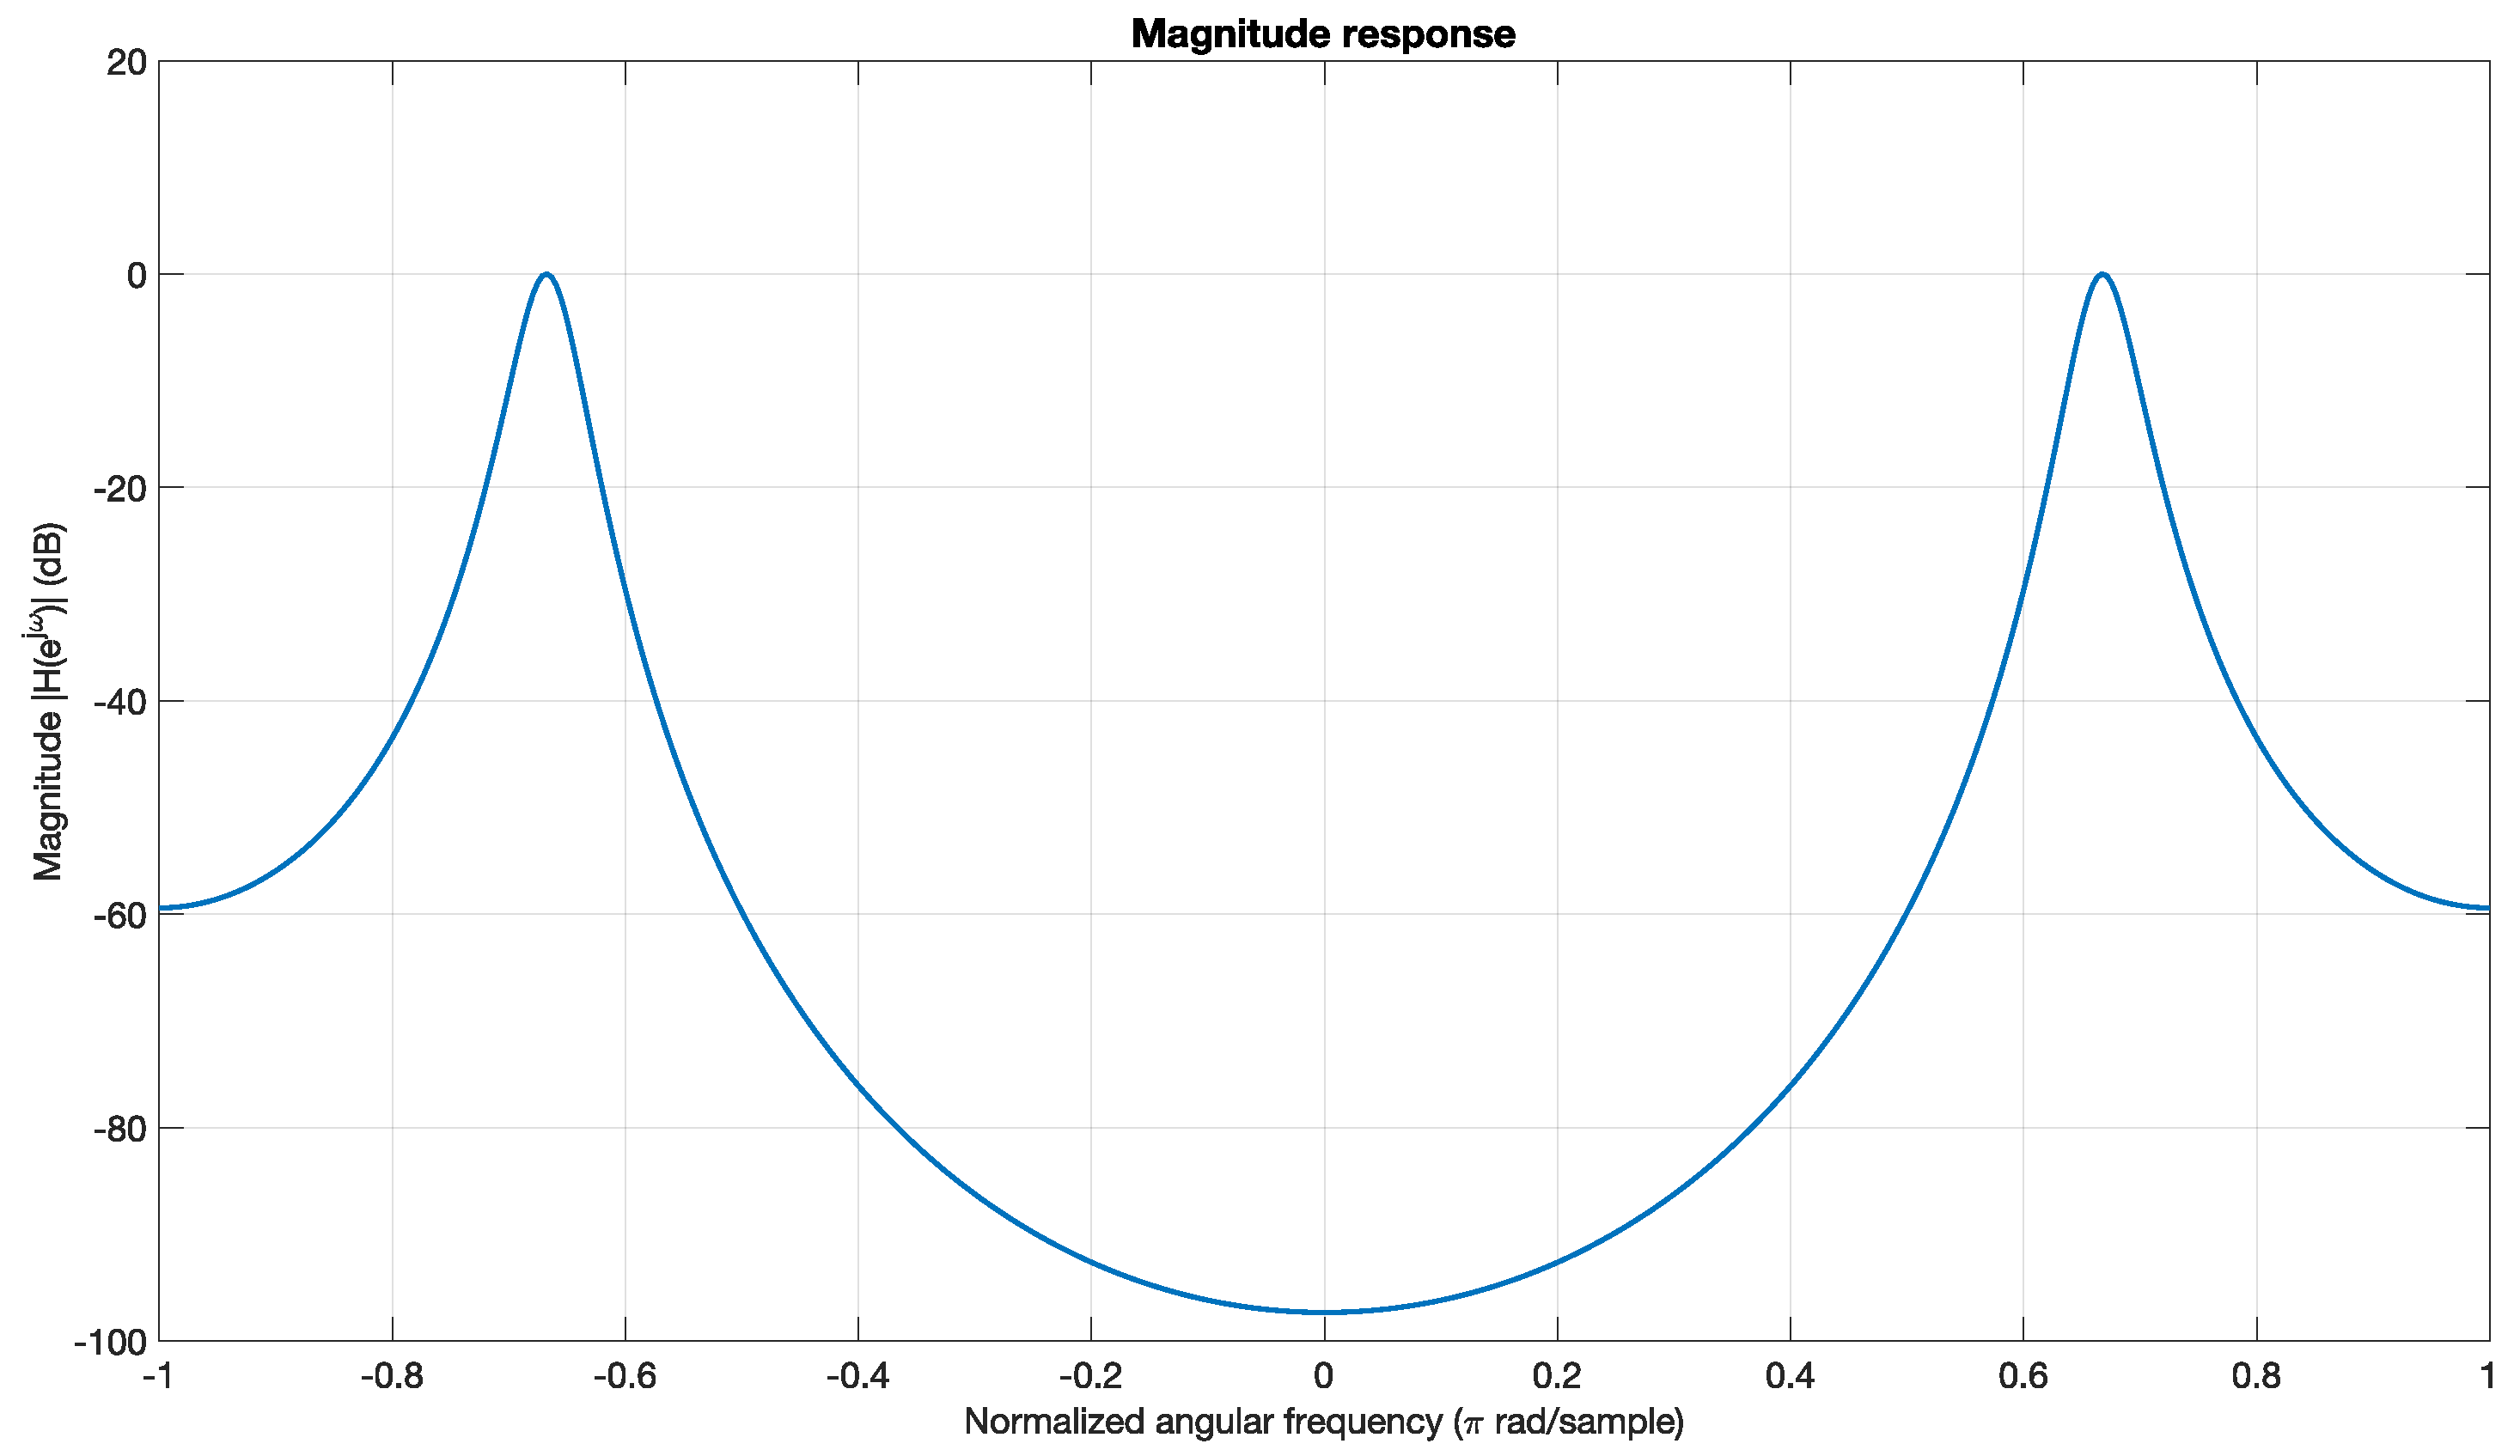
\includegraphics[width=1\textwidth]{resources/pdf/magnitude_response_b.pdf}
	    \caption{Magnitude response $\abs{H(e^{j\omega})}$ for $\omega_0 = \frac{2\pi}{3}$.}
	    \label{fig:magnitude_response_b}
	\end{figure}
	Examining figures \ref{fig:magnitude_response_a} and \ref{fig:magnitude_response_b}, we found that it is a band-pass filter. Indeed, this filter passes only a frequency band around the value $\omega_0$.\par
	By varying the value of this parameter $\omega_0$, we observe that the band-pass filter does not let the same frequency band pass.\par
	In conclusion, the impact of the change of the parameter $\omega_0$ is implicit. This defines which frequency band the filter will pass.
	\newpage
	\section{Autocorrelation of a single echo}
	Let the expression of a single echo $y[n]$ generated using the FIR filter
	\begin{equation}
	    \label{eq:echo_y}
	    \tag{$\dagger$}
	    y[n] = x[n] + ax[n-D],\quad -1<a<1
	\end{equation}
	By definition, the expression of the autocorrelation $r_y[l]$ is given by
	\begin{equation*}
	    r_y[l] = \sum_{n=-\infty}^{\infty}y[n]\times y[n-l]
	\end{equation*}
	We can replace $y[n]$ by its expression \eqref{eq:echo_y}
	\begin{equation*}
	    r_y[l] = \sum_{n=-\infty}^{\infty}(x[n]+ax[n-D])\times (x[n-l] + ax[n-l-D])
	\end{equation*}
	By distributing, we get
	\begin{align*}
	    r_y[l] &= \sum_{n=-\infty}^{\infty}(a_1+a_2+a_3+a_4)\\
	    &= \sum_{n=-\infty}^{\infty}a_1 + \sum_{n=-\infty}^{\infty}a_2 + \sum_{n=-\infty}^{\infty}a_3 + \sum_{n=-\infty}^{\infty}a_4
	\end{align*}
	where
	\begin{itemize}
	    \item $a_1 = x[n]\times x[n-l]$
	    \item $a_2 = x[n]\times ax[n-l-D]$
	    \item $a_3 = ax[n-D]\times x[n-l] = ax[n-D]\times x[n-D-\rbk{l-D}]$
	    \item $a_4 = ax[n-D]\times ax[n-l-D]$
	\end{itemize}
	We note that we fall back on the definition of the autocorrelation of the signal $x$. By replacing the terms with this definition, we find the expression of the autocorrelation $r_y[l]$ in terms of the autocorrelation $r_x[l]$, $D$ and $a$
	\begin{align*}
	    r_y[l] &= r_x[l] + ar_x[l+D] + ar_x[l-D] + a^2r_x[l]\\
	    &= (1+a^2)r_x[l] + a\rbk{r_x[l-D] + r_x[l+D]}
	\end{align*}
	\newpage
	\section{Echo cancellation}
	Using the \texttt{audioread} and \texttt{xcorr} functions of Matlab, we play the sound and plot its autocorrelation function (figure \ref{fig:sound_autocorrelation}).\par
	\begin{figure}[!ht]
	    \centering
	    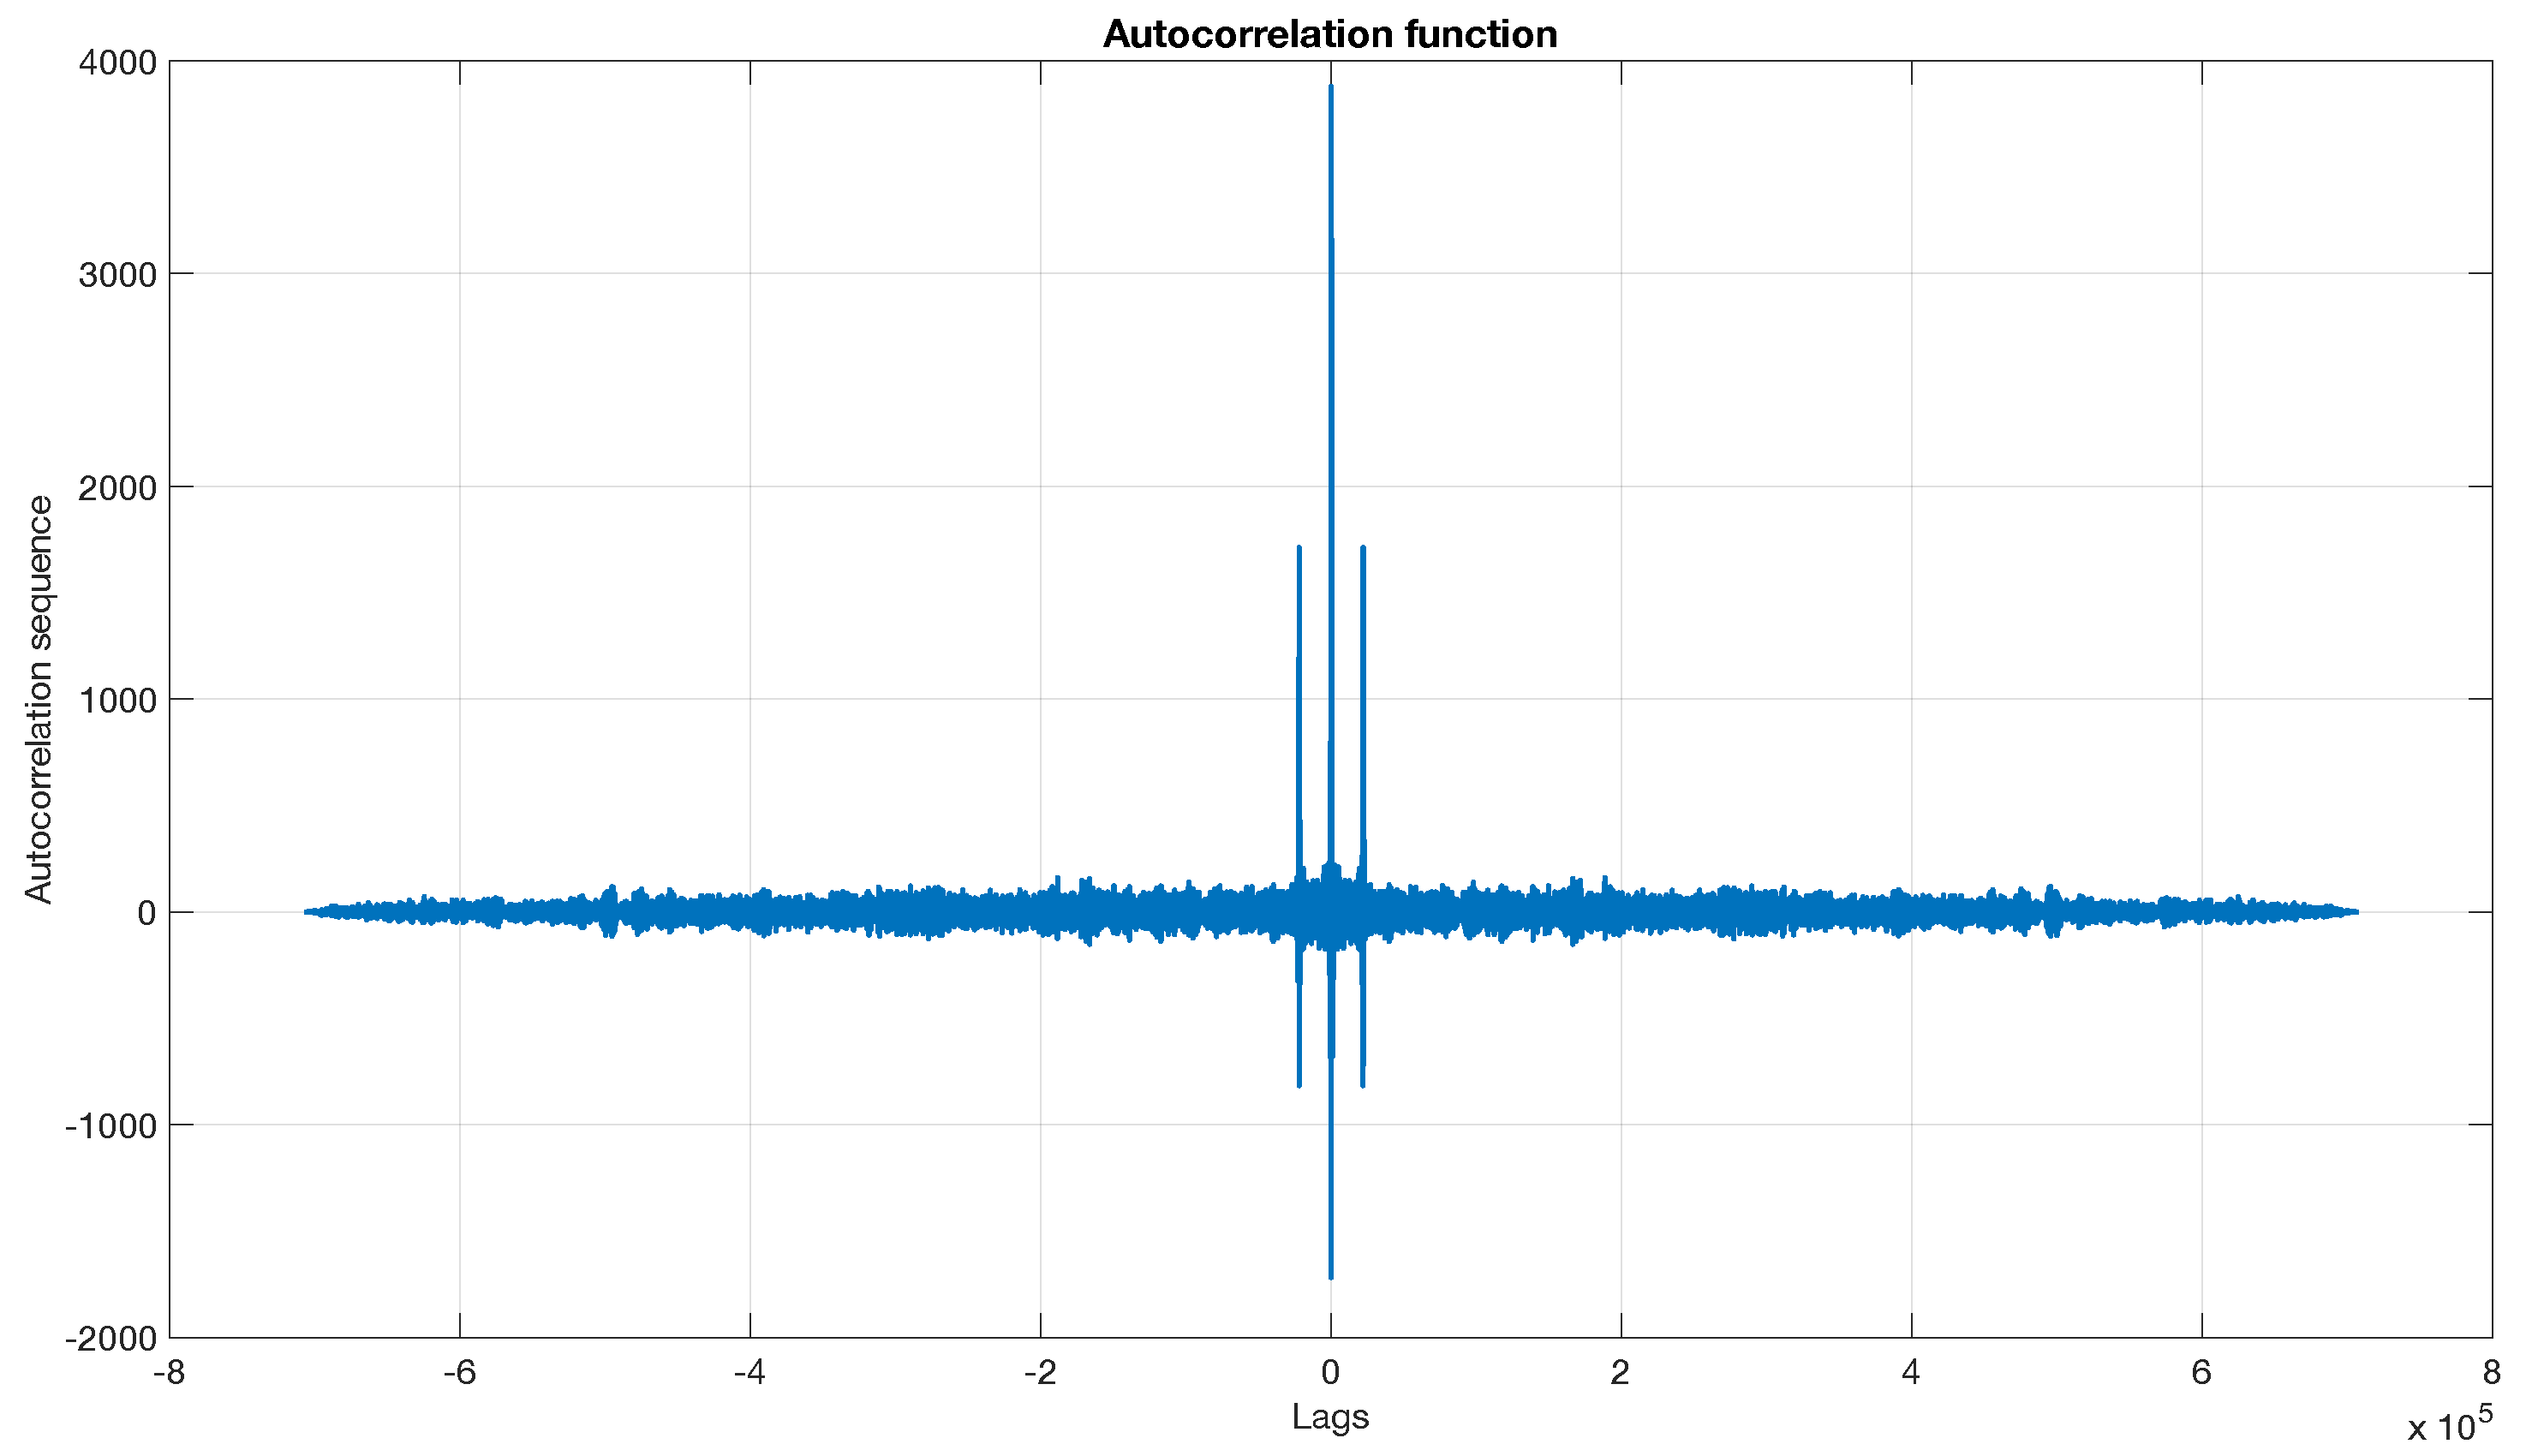
\includegraphics[width=1\textwidth]{resources/pdf/sound_autocorrelation.pdf}
	    \caption{Autocorrelation function of the sound \texttt{hw1\_echo.wav}.}
	    \label{fig:sound_autocorrelation}
	\end{figure}
	The expression of the signal with echo is given by
	\begin{equation*}
	    y(n) = x(n) + \alpha x(n-d)
	\end{equation*}
	with $x(n)$, the original sound without echo. The goal is to recover $x(n)$.\par
	By passing into the frequency domain, we have
	\begin{equation*}
	    Y(z) = X(z) + \alpha X(z)z^{-d}
	\end{equation*}
	We can find the transfer function
	\begin{align*}
	    H(z) &= \dfrac{Y(z)}{X(z)}\\
	    &= 1 + \alpha z^{-d}
	\end{align*}
	And so, we have
	\begin{equation*}
	    X(z) = \dfrac{Y(z)}{H(z)}
	\end{equation*}
	This means that we need to filter the observed signal $y(n)$ through the filter $\frac{1}{H(z)}$ in order to recover $x(n)$. To build the transfer function, we have to find the delay $d$.\par
	In the figure \ref{fig:sound_autocorrelation}, several peaks are observed. The delay can be found by observing the distance between two consecutive peaks.\par
	We thus find the delay (expressed in number of sampling intervals) $d = \num{2.205e4}$. We can also find the corresponding delay expressed in seconds by divising this value by \texttt{fs}. We obtain (in seconds): $\tau = \num{0.5}$.\par
	We assume that the amplitude of the reflected sound is sixty percent of the emitted one, so $\alpha = 0.6$. We can now build the coefficients of the transfer function. These are stored in the vectors $b$ (for the numerator) and $a$ (for the denominator).\par
	Now just call the function \texttt{filter} of Matlab with as arguments the vectors containing the coefficients and the sound to be filtered. The new sound obtained can be played with the function \texttt{sound} of Matlab. It can be seen that it no longer contains an echo.
	\newpage
	\appendix
	\section{Matlab codes}
	\subsection{Magnitude response of a filter}
	\lstinputlisting[style=NFmatlab]{resources/m/Q1.m}
	\subsection{Echo cancellation}
	\lstinputlisting[style=NFmatlab]{resources/m/Q3.m}
\end{document}
